\lecture{虚函数与多态性}{lec:chap06}
\section[虚函数]{虚函数}\label{sec:chap06-sec01}
%%%%%%%%%%%%%%%%%%%%%%%%%%%%%% 继承与派生的概念 %%%%%%%%%%%%%%%%%%%%%%%%%%%%%%%%%%
\begin{frame}[t, fragile]{虚函数}{为何引入虚函数?}%
  \stretchon
  \begin{itemize}
  \item 为派生类提供一致的接口(Uniform Interface)
  \item \alert{多态性}:同一消息发送给不同对象执行不同操作
  \end{itemize}
  \stretchoff
\end{frame}

\begin{frame}[t, fragile]{虚函数}{动物园类}%
  \stretchon
  \begin{itemize}
  \item 设计一个动物园类
    \begin{itemize}
    \item 包含大量不同种类的动物
    \item 可以显示各种动物的属性(如名字、年龄等)
    \item 可以输出各种动物的叫声
    \end{itemize}
  \end{itemize}
  \stretchoff
\end{frame}

\begin{frame}[t, fragile]{虚函数}{动物园类}%
  \begin{itemize}
  \item 设计一个动物园类    
  \end{itemize}
  \begin{center}
     \begin{tikzpicture}[font=\tiny, show background grid]
      \tikzset{ coord/.style={coordinate} }

      \begin{class}[fill=red!25, text width=4em]{动物类CAnimal}{0, 0}

      \end{class}

      \begin{class}[fill=green!25, text width=4em]{马CHorse}{-3, -2}
        \inherit{动物类CAnimal}

      \end{class}
      
      \begin{class}[fill=green!25, text width=4em]{鸟CBird}{0, -2}
        \inherit{动物类CAnimal}

      \end{class}
      
      \begin{class}[fill=green!25, text width=4em]{牛类CBull}{3, -2}
        \inherit{动物类CAnimal}

      \end{class}

      \begin{class}[fill=blue!25, text width=4em]{飞马CPegasus}{-1.5, -4}
        \inherit{马CHorse}
        \inherit{鸟CBird}

      \end{class}
           
    \end{tikzpicture}    
  \end{center}
\end{frame}

\begin{frame}[t, fragile]{虚函数}{动物园类}%
  \begin{itemize}
  \item 设计一个动物园类    
  \end{itemize}
  \begin{center}
     \begin{tikzpicture}[font=\tiny, show background grid]
      \tikzset{ coord/.style={coordinate} }

      \node[anchor=north west] (fig1) at (0,0)
      {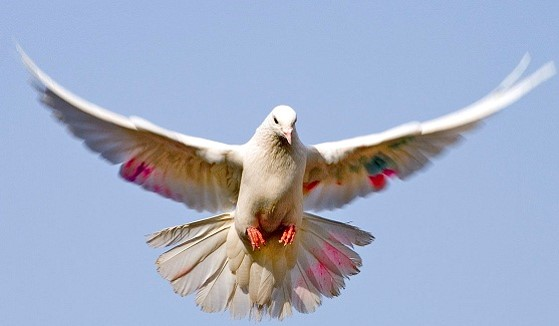
\includegraphics[width=0.25\textwidth]{figure/chap06/01bird}};

      \node[anchor=north west, right=0.5 of fig1] (fig2)
      {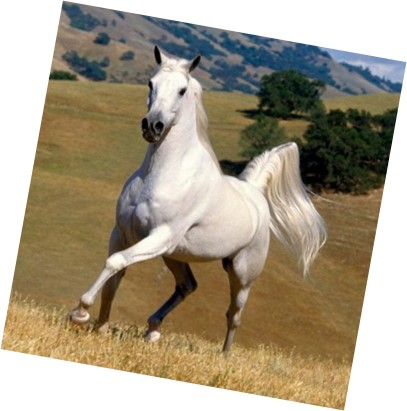
\includegraphics[width=0.25\textwidth]{figure/chap06/02horse}};

      \node[anchor=north west, below=0.5 of fig1] (fig3)
      {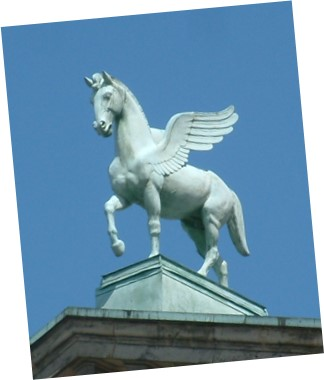
\includegraphics[width=0.2\textwidth]{figure/chap06/03pegasus}};

      \node[anchor=north west, below=0.5 of fig2] (fig4)
      {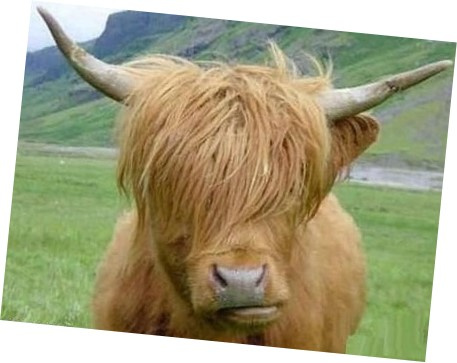
\includegraphics[width=0.25\textwidth]{figure/chap06/04bull}};
           
    \end{tikzpicture}    
  \end{center}
\end{frame}

\begin{frame}[t, fragile]{虚函数}{动物园类}%
  \begin{itemize}
  \item 设计一个动物园类    
  \end{itemize}
  \begin{center}
     \begin{tikzpicture}[font=\tiny, show background grid]
      \tikzset{ coord/.style={coordinate} }

      \begin{class}[fill=red!25, text width=4em]{动物类CAnimal}{0, 0}
        \attribute{-name[32]:char}
        \attribute{-age:int}
        \attribute{-weight:int}
        \operation{+show():void}
      \end{class}

      \begin{class}[fill=green!25, text width=4em]{马CHorse}{-3, -2.5}
        \inherit{动物类CAnimal}
        \attribute{-power:int}
        \operation{+show():void}
        \operation{+talk():void}
      \end{class}
      
      \begin{class}[fill=green!25, text width=4em]{鸟CBird}{0, -2.5}
        \inherit{动物类CAnimal}
        \attribute{-wingSpan:int}
        \operation{+show():void}
        \operation{+talk():void}
      \end{class}
      
      \begin{class}[fill=green!25, text width=4em]{牛CBull}{3, -2.5}
        \inherit{动物类CAnimal}
        \attribute{-power:int}
        \operation{+show():void}
        \operation{+talk():void}
      \end{class}

      \begin{class}[fill=blue!25, text width=4em]{飞马CPegasus}{-1.5, -5}
        \inherit{马CHorse}
        \inherit{鸟CBird}
        \operation{+show():void}
        \operation{+talk():void}
      \end{class}
           
    \end{tikzpicture}    
  \end{center}
\end{frame}

\begin{frame}[t, fragile]{虚函数}{动物园类}%
  \begin{itemize}
  \item 设计一个动物园类    
  \end{itemize}
  \begin{center}
    \begin{tikzpicture}[font=\tiny, show background grid]
      \tikzset{ coord/.style={coordinate} }
      
      \umlnote[text width=0.8\textwidth](note1) at (0, 0)
      {
        \cppfilenobg{codes/chap06/01-zoo-CAnimal.cpp}
      };
      
    \end{tikzpicture}
  \end{center}
\end{frame}

\begin{frame}[t, fragile]{虚函数}{动物园类}%
  \begin{itemize}
  \item 设计一个动物园类    
  \end{itemize}
  \begin{center}
    \begin{tikzpicture}[font=\tiny, show background grid]
      \tikzset{ coord/.style={coordinate} }
      
      \umlnote[text width=0.8\textwidth](note1) at (0, 0)
      {
        \cppfilenobg{codes/chap06/01-zoo-CBird.cpp}
      };

      \path let \p1=(note1) in
      coordinate (org) at (\x1, \y1)
      coordinate (ovBL1) at ($(org) + (-4.70, -2.10)$)
      coordinate (ovUR1) at ($(ovBL1) + (2.80, -0.30)$)
      ;

      \draw[red,thick,fill=green!35, fill opacity=0.3](ovBL1) rectangle
      (ovUR1);
      
    \end{tikzpicture}
  \end{center}
\end{frame}

\begin{frame}[t, fragile]{虚函数}{动物园类}%
  \begin{itemize}
  \item 设计一个动物园类    
  \end{itemize}
  \begin{center}
    \begin{tikzpicture}[font=\tiny, show background grid]
      \tikzset{ coord/.style={coordinate} }
      
      \umlnote[text width=0.8\textwidth](note1) at (0, 0)
      {
        \cppfilenobg{codes/chap06/01-zoo-CHorse.cpp}
      };

      \path let \p1=(note1) in
      coordinate (org) at (\x1, \y1)
      coordinate (ovBL1) at ($(org) + (-4.70, -2.10)$)
      coordinate (ovUR1) at ($(ovBL1) + (2.90, -0.30)$)
      ;

      \draw[red,thick,fill=green!35, fill opacity=0.3](ovBL1) rectangle
      (ovUR1);
      
    \end{tikzpicture}
  \end{center}
\end{frame}

\begin{frame}[t, fragile]{虚函数}{动物园类}%
  \begin{itemize}
  \item 设计一个动物园类    
  \end{itemize}
  \begin{center}
    \begin{tikzpicture}[font=\tiny, show background grid]
      \tikzset{ coord/.style={coordinate} }
      
      \umlnote[text width=0.9\textwidth](note1) at (0, 0)
      {
        \cppfilenobg{codes/chap06/01-zoo-CPegasus.cpp}
      };

      \path let \p1=(note1) in
      coordinate (org) at (\x1, \y1)
      coordinate (ovBL1) at ($(org) + (-5.30, -2.25)$)
      coordinate (ovUR1) at ($(ovBL1) + (1.60, -0.30)$)
      ;

      \draw[red,thick,fill=green!35, fill opacity=0.3](ovBL1) rectangle
      (ovUR1);
      
    \end{tikzpicture}
  \end{center}
\end{frame}

\begin{frame}[t, fragile]{虚函数}{动物园类}%
  \begin{itemize}
  \item 设计一个动物园类    
  \end{itemize}
  \begin{center}
    \begin{tikzpicture}[font=\tiny, show background grid]
      \tikzset{ coord/.style={coordinate} }
      
      \umlnote[text width=0.8\textwidth](note1) at (0, 0)
      {
        \cppfilenobg{codes/chap06/01-zoo-CBull.cpp}
      };

      \path let \p1=(note1) in
      coordinate (org) at (\x1, \y1)
      coordinate (ovBL1) at ($(org) + (-4.70, -1.98)$)
      coordinate (ovUR1) at ($(ovBL1) + (2.60, -0.3)$)
      ;

      \draw[red,thick,fill=green!35, fill opacity=0.3](ovBL1) rectangle
      (ovUR1);
      
    \end{tikzpicture}
  \end{center}
\end{frame}

\begin{frame}[t, fragile]{虚函数}{动物园类}%
  \begin{itemize}
  \item 设计一个动物园类    
  \end{itemize}
  \begin{center}
    \begin{tikzpicture}[font=\tiny, show background grid]
      \tikzset{ coord/.style={coordinate} }
      
      \umlnote[text width=0.8\textwidth](note1) at (0, 0)
      {
        \cppfilenobg{codes/chap06/01-zoo-main.cpp}
      };
      
    \end{tikzpicture}
  \end{center}
\end{frame}

\begin{frame}[t, fragile]{虚函数}{动物园类}%
  \begin{itemize}
  \item 如果有大量的不同种类的动物,如何进行管理?
  \item 设计一个动物园类
  \end{itemize}
  \begin{center}
    \begin{tikzpicture}[font=\tiny, show background grid]
      \tikzset{ coord/.style={coordinate} }
      
      \umlnote[text width=0.8\textwidth](note1) at (0, 0)
      {
        \cppfilenobg{codes/chap06/02-zoo.cpp}
      };
      
    \end{tikzpicture}
  \end{center}  
\end{frame}

\begin{frame}[t, fragile]{虚函数}{动物园类}%
  \begin{itemize}
  \item 多种动物    
  \end{itemize}
  \begin{center}
    \begin{tikzpicture}[font=\tiny, show background grid]
      \tikzset{ coord/.style={coordinate} }
      
      \umlnote[text width=0.4\textwidth](code1) at (0, 0)
      {
        \cppfilenobg{codes/chap06/02-zoo-show.cpp}
      };

      \umlnote[text width=0.4\textwidth, right=0.5 of code1](code2)
      {
        \cppfilenobg{codes/chap06/02-zoo-talk.cpp}
      };
      
    \end{tikzpicture}
  \end{center}
\end{frame}

\begin{frame}[t, fragile]{虚函数}{动物园类}%
  \begin{itemize}
  \item 缺点:对具有相同基类的派生类对象需要分别设计
  \item 若派生类数量增加,管理复杂度上升
  \end{itemize}
  \begin{center}
    \begin{tikzpicture}[font=\tiny, show background grid]
      \tikzset{ coord/.style={coordinate} }
      
      \umlnote[text width=0.8\textwidth](note1) at (0, 0)
      {
        \cppfilenobg{codes/chap06/02-zoo.cpp}
      };
      
    \end{tikzpicture}
  \end{center}  
\end{frame}

\begin{frame}[t, fragile]{虚函数}{动物园类}%
  \begin{itemize}
  \item 另外一种考虑方式:\alert{类型兼容}
  \end{itemize}
  \begin{center}
    \begin{tikzpicture}[font=\tiny, show background grid]
      \tikzset{ coord/.style={coordinate} }
      
      \umlnote[text width=0.4\textwidth](code1) at (0, 0)
      {
        \cppfilenobg{codes/chap06/03-zoo-class.cpp}
      };

      \umlnote[text width=0.35\textwidth, right=0.3 of code1](code2)
      {
        \cppfilenobg{codes/chap06/03-zoo-show-talk.cpp}
      };

      \node[anchor=north west, text width=0.35\textwidth, below=0.3 of code2] (fig1)
      {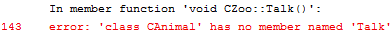
\includegraphics[width=1.0\textwidth]{figure/chap06/05virtualfunerror}};

      \path let \p1=(code1) in
      coordinate (code10) at (\x1, \y1)
      coordinate (ovfun10) at ($(code10) + (-1.9, -0.56)$)
      coordinate (ovfun11) at ($(ovfun10) + (2.0, 0)$)
      coordinate (ovfunc1) at ($(ovfun10)!0.5!(ovfun11)$)
      ;

      \path let \p1=(code2) in
      coordinate (code20) at (\x1, \y1)
      coordinate (ovfun20) at ($(code20) + (-1.70, -1.82)$)
      coordinate (ovfun21) at ($(ovfun20) + (2.05, 0)$)
      coordinate (ovfunc2) at ($(ovfun20)!0.5!(ovfun21)$)
      ;

      \draw[red, thick] (ovfun10) -- (ovfun11);
      \draw[red, thick] (ovfun20) -- (ovfun21);

      \draw[-{Stealth[scale=1.0]}, blue, thick] (ovfun21) to[out=0,
      in=0] (fig1.east);
      % \draw[-{Stealth[scale=1.0]}, red, thick] (ovfunc1) to[out=-90,
      % in=-90] (ovfunc3);
      
    \end{tikzpicture}
  \end{center}
\end{frame}

\begin{frame}[t, fragile]{虚函数}{动物园类}%
  \begin{itemize}
  \item 问题1:基类不能调用派生类成员函数Talk
  \item 解决办法:\alert{虚函数}
  \end{itemize}
  \begin{center}
    \begin{tikzpicture}[font=\tiny, show background grid]
      \tikzset{ coord/.style={coordinate} }
      
      \umlnote[text width=0.4\textwidth](code1) at (0, 0)
      {
        \cppfilenobg{codes/chap06/04-zoo-virtfun-show.cpp}
      };

      \umlnote[text width=0.4\textwidth, right=0.3 of code1](code2)
      {
        \cppfilenobg{codes/chap06/04-zoo-virtfun-talk.cpp}
      };

      \path let \p1=(code1) in
      coordinate (org) at (\x1, \y1)
      coordinate (ovBL1) at ($(org) + (-2.65, 0.2)$)
      coordinate (ovUR1) at ($(ovBL1) + (0.85, -0.3)$)
      ;

      \path let \p1=(code2) in
      coordinate (org) at (\x1, \y1)
      coordinate (ovBL2) at ($(org) + (-2.65, 0.03)$)
      coordinate (ovUR2) at ($(ovBL2) + (0.85, -0.3)$)
      ;

      \draw[red,thick,fill=green!35, fill opacity=0.3](ovBL1) rectangle
      (ovUR1);
      \draw[red,thick,fill=green!35, fill opacity=0.3](ovBL2) rectangle
      (ovUR2);  
      
    \end{tikzpicture}
  \end{center}
\end{frame}

\begin{frame}[t, fragile]{虚函数}{动物园类}%
  \begin{itemize}
  \item 问题1:基类不能调用派生类成员函数Talk
  \item 解决办法:\alert{虚函数}
  \end{itemize}
  \begin{center}
    \begin{tikzpicture}[font=\tiny, show background grid]
      \tikzset{ coord/.style={coordinate} }
      
      \umlnote[text width=0.6\textwidth](code1) at (0, 0)
      {
        \cppfilenobg{codes/chap06/04-zoo-main.cpp}
      };      

      \path let \p1=(code1) in
      coordinate (org) at (\x1, \y1)
      coordinate (ovBL1) at ($(org) + (-3.7, 0.32)$)
      coordinate (ovUR1) at ($(ovBL1) + (1.0, -0.3)$)
      ;

      \path let \p1=(code1) in
      coordinate (org) at (\x1, \y1)
      coordinate (ovBL2) at ($(org) + (-3.7, -1.26)$)
      coordinate (ovUR2) at ($(ovBL2) + (2.0, 1.1)$)
      ;

      \path let \p1=(code1) in
      coordinate (org) at (\x1, \y1)
      coordinate (ovBL3) at ($(org) + (-3.7, -2.05)$)
      coordinate (ovUR3) at ($(ovBL3) + (1.35, 0.55)$)
      ;

      \draw[red,thick,fill=green!35, fill opacity=0.3](ovBL1) rectangle
      (ovUR1);
      \draw[blue,thick,fill=red!35, fill opacity=0.3](ovBL2) rectangle
      (ovUR2);
      \draw[green,thick,fill=blue!35, fill opacity=0.3](ovBL3) rectangle
      (ovUR3);
      
    \end{tikzpicture}
  \end{center}
\end{frame}

\begin{frame}[t, fragile]{虚函数}{基本语法}%
  \begin{spacing}{1.8}
  \begin{itemize}
  \item 定义\\
    \begin{center}
      \begin{minipage}[t]{0.5\linewidth}
        \begin{cppttnobg}
virtual |函数类型| |函数表|(|形参表|)
{
  |函数体|;
}
        \end{cppttnobg}
      \end{minipage}
    \end{center}        
    \begin{itemize}
    \item 只有类的成员函数才能声明为虚函数
    \item 虚函数不能是静态成员函数,也不能是友元函数
    \item 若在基类中定义虚函数,在派生类中还需重新定义
    \item 构造函数不能是虚函数,析构函数可以是虚函数
    \end{itemize}    
  \end{itemize}
  \end{spacing}
\end{frame}

\begin{frame}[t, fragile]{虚函数}{虚析构函数}%
  \begin{itemize}
  \item 定义\\    
      \begin{center}
      \begin{minipage}[t]{0.5\linewidth}
        \begin{cppttnobg}
virtual ~|类名|()
{
  |函数体|;
}
        \end{cppttnobg}
      \end{minipage}
    \end{center}
  \end{itemize}
\end{frame}

\begin{frame}[t, fragile]{虚函数}{虚析构函数}%
  \begin{itemize}
  \item 虚析构函数
  \end{itemize}
  \vspace{-3ex}
  \begin{center}
    \begin{tikzpicture}[font=\tiny, show background grid]
      \tikzset{ coord/.style={coordinate} }
      
      \umlnote[scale = 0.90, text width=0.45\textwidth](code1) at (0, 0)
      {
        \cppfilenobg{codes/chap06/05-dtor-base.cpp}
      };

      \umlnote[scale = 0.90, text width=0.45\textwidth, right=0.3 of code1](code2)
      {
        \cppfilenobg{codes/chap06/05-dtor-derived.cpp}
      };

      \umlnote[scale = 0.90, text width=0.45\textwidth, below=0.1 of code1](code3)
      {
        \cppfilenobg{codes/chap06/05-dtor-main.cpp}
      };

      \node[text width=0.35\textwidth, below=0.1 of code2] (fig1)
      {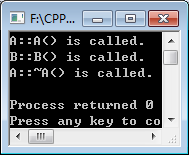
\includegraphics[width=0.5\textwidth]{figure/chap06/06novdtor}};

      \path let \p1=(code1) in
      coordinate (org) at (\x1, \y1)
      coordinate (ovBL0) at ($(org) + (-2.45, 0.37)$)
      coordinate (ovUR0) at ($(ovBL0) + (1.35, -0.3)$)
      coordinate (ovBR0) at ($(ovBL0) + (0.0, -0.3)$)
      coordinate (ovfunc0) at ($(ovUR0)!0.5!(ovBR0)$)
      ;

      \path let \p1=(code2) in
      coordinate (org) at (\x1, \y1)
      coordinate (ovBL1) at ($(org) + (-2.45, -0.85)$)
      coordinate (ovUR1) at ($(ovBL1) + (1.35, -0.3)$)
      coordinate (ovUL1) at ($(ovBL1) + (0.0, -0.3)$)
      coordinate (ovfunc1) at ($(ovBL1)!0.5!(ovUL1)$)
      ;

      \path let \p1=(code3) in
      coordinate (org) at (\x1, \y1)
      coordinate (ovBL2) at ($(org) + (-2.50, -0.20)$)
      coordinate (ovUR2) at ($(ovBL2) + (1.1, -0.3)$)
      coordinate (ovUL2) at ($(ovBL2) + (1.1, 0.0)$)
      coordinate (ovfunc2) at ($(ovUL2)!0.5!(ovUR2)$)
      ;

      \draw[blue,thick,fill=red!35, fill opacity=0.3](ovBL0) rectangle
      (ovUR0);
      \draw[red,thick,fill=green!35, fill opacity=0.3](ovBL1) rectangle
      (ovUR1);
      \draw[red,thick,fill=green!35, fill opacity=0.3](ovBL2) rectangle
      (ovUR2);

      \draw[-{Stealth[scale=1.0]}, blue, thick] (ovfunc2) to[out=0,
      in=180] (fig1.west);
      \draw[-{Stealth[scale=1.0]}, blue, thick] (ovfunc2) to[out=0,
      in=-90] node [above=1mm]
      {\textcircled{2}} (ovfunc0);
      \draw[-{Stealth[scale=1.0]}, red, thick] (ovfunc2) to[out=0,
      in=180] node [above=1mm]
      {\textcircled{1} \large \badmark} (ovfunc1);
      % \draw[-{Stealth[scale=1.0]}, red, thick] (ovfunc1) to[out=180,
      % in=-90] (ovfunc0);
      
    \end{tikzpicture}
  \end{center}
\end{frame}

\begin{frame}[t, fragile]{虚函数}{虚析构函数}%
  \begin{itemize}
  \item 虚析构函数
  \end{itemize}
  \vspace{-3ex}
  \begin{center}
    \begin{tikzpicture}[font=\tiny, show background grid]
      \tikzset{ coord/.style={coordinate} }
      
      \umlnote[scale = 0.90, text width=0.45\textwidth](code1) at (0, 0)
      {
        \cppfilenobg{codes/chap06/06-vdtor-base.cpp}
      };

      \umlnote[scale = 0.90, text width=0.45\textwidth, right=0.3 of code1](code2)
      {
        \cppfilenobg{codes/chap06/05-dtor-derived.cpp}
      };

      \umlnote[scale = 0.90, text width=0.45\textwidth, below=0.1 of code1](code3)
      {
        \cppfilenobg{codes/chap06/05-dtor-main.cpp}
      };

      \node[text width=0.35\textwidth, below=0.2 of code2] (fig1)
      {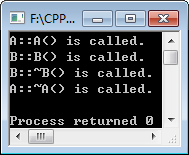
\includegraphics[width=0.5\textwidth]{figure/chap06/07vdtor}};

      \path let \p1=(code1) in
      coordinate (org) at (\x1, \y1)
      coordinate (ovBL0) at ($(org) + (-2.45, 0.37)$)
      coordinate (ovUR0) at ($(ovBL0) + (1.35, -0.3)$)
      coordinate (ovBR0) at ($(ovBL0) + (0.0, -0.3)$)
      coordinate (ovfunc0) at ($(ovUR0)!0.5!(ovBR0)$)
      ;

      \path let \p1=(code2) in
      coordinate (org) at (\x1, \y1)
      coordinate (ovBL1) at ($(org) + (-2.45, -0.85)$)
      coordinate (ovUR1) at ($(ovBL1) + (1.35, -0.3)$)
      coordinate (ovUL1) at ($(ovBL1) + (0.0, -0.3)$)
      coordinate (ovfunc1) at ($(ovBL1)!0.5!(ovUL1)$)
      ;

      \path let \p1=(code3) in
      coordinate (org) at (\x1, \y1)
      coordinate (ovBL2) at ($(org) + (-2.50, -0.20)$)
      coordinate (ovUR2) at ($(ovBL2) + (1.1, -0.3)$)
      coordinate (ovUL2) at ($(ovBL2) + (1.1, 0.0)$)
      coordinate (ovfunc2) at ($(ovUL2)!0.5!(ovUR2)$)
      ;

      \draw[blue,thick,fill=red!35, fill opacity=0.3](ovBL0) rectangle
      (ovUR0);
      \draw[red,thick,fill=green!35, fill opacity=0.3](ovBL1) rectangle
      (ovUR1);
      \draw[red,thick,fill=green!35, fill opacity=0.3](ovBL2) rectangle
      (ovUR2);

      \draw[-{Stealth[scale=1.0]}, blue, thick] (ovfunc2) to[out=0,
      in=180] (fig1.west);
      \draw[-{Stealth[scale=1.0]}, blue, thick] (ovfunc2) to[out=0,
      in=-90] node [above=1mm]
      {\textcircled{2}} (ovfunc0);
      \draw[-{Stealth[scale=1.0]}, red, thick] (ovfunc2) to[out=0,
      in=180] node [above=1mm]
      {\textcircled{1}} (ovfunc1);
      
    \end{tikzpicture}
  \end{center}
\end{frame}

\begin{frame}[t, fragile]{虚函数}{虚析构函数}%
  \begin{spacing}{1.6}
  \begin{itemize}
  \item 定义基类的析构函数是虚析构函数,当程序运行结束时,通过基类指针删除派生类对象时,先调用派生类析构函数,然后调用基类析构函数
  \end{itemize}
  \end{spacing}
\end{frame}

%%%%%%%%%%%%%%%%%%%%%%%%%%%%%%%%%%%%%%%%%%%%%%%%%%%%%%%%%%%%%%%%%%%%%%%%%%%%%%%

\section[抽象类]{抽象类}\label{sec:chap06-sec02}
%%%%%%%%%%%%%%%%%%%%%%%%%%%%%% 继承的方式 %%%%%%%%%%%%%%%%%%%%%%%%%%%%%%%%%%
\begin{frame}[t, fragile]{抽象类}{纯虚函数和抽象类}%
  \begin{itemize}
  \item 纯虚函数定义\\    
    \begin{center}
      \begin{minipage}[t]{0.5\linewidth}
        \begin{cppttnobg}
virtual |函数类型| |函数名|(|参数表|)|\textcolor{red}{=0}|;
        \end{cppttnobg}
      \end{minipage}
    \end{center}
  \item 抽象类定义
    \begin{itemize}
    \item 类中含有至少一个纯虚函数
    \end{itemize}
  \end{itemize}
\end{frame}

\begin{frame}[t, fragile]{抽象类}{纯虚函数和抽象类}%
  \begin{itemize}
  \item 回顾动物类中的虚函数Talk→函数体无意义\\    
    \begin{center}
      \begin{minipage}[t]{0.5\linewidth}
        \begin{cppttnobg}
virtual void CAnimal::Talk()
{
  cout << "Do nothing!" << endl;
}
        \end{cppttnobg}
      \end{minipage}
    \end{center}
  \item 解决办法:\alert{纯虚函数}\\
    \begin{center}
      \begin{minipage}[t]{0.5\linewidth}
        \begin{cppttnobg}
virtual void CAnimal::Talk() = 0;
        \end{cppttnobg}
      \end{minipage}
    \end{center}
  \end{itemize}
\end{frame}

\begin{frame}[t, fragile]{抽象类}{纯虚函数和抽象类}%
  \begin{itemize}
  \item 不能实例化(不能创建类的对象)
  \end{itemize}
  \begin{center}
    \begin{tikzpicture}[font=\tiny, show background grid]
      \tikzset{ coord/.style={coordinate} }
      
      \umlnote[text width=0.35\textwidth](code1) at (0, 0)
      {
        \cppfilettnobg{codes/chap06/07-abstract-main.cpp}
      };

      \node[text width=0.8\textwidth, below=0.2 of code1] (fig1)
      {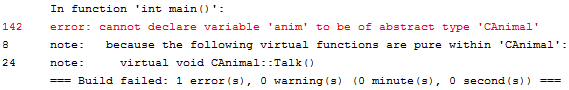
\includegraphics[width=1.0\textwidth]{figure/chap06/08abstractobj}};

      \path let \p1=(code1) in
      coordinate (org) at (\x1, \y1)
      coordinate (ovBL0) at ($(org) + (-2.05, 0.28)$)
      coordinate (ovUR0) at ($(ovBL0) + (2.15, -0.3)$)
      coordinate (ovBR0) at ($(ovBL0) + (0.0, -0.3)$)
      coordinate (ovfunc0) at ($(ovUR0)!0.5!(ovBR0)$)
      ;

      \draw[blue,thick,fill=red!35, fill opacity=0.3](ovBL0) rectangle
      (ovUR0);
    \end{tikzpicture}
  \end{center}  
\end{frame}

\begin{frame}[t, fragile]{抽象类}{实例:甜甜圈小屋}%
  \begin{itemize}
  \item 例子: 甜甜圈小屋分析
  \end{itemize}
  \begin{center}
    \begin{tikzpicture}[font=\tiny, show background grid]
      \tikzset{ coord/.style={coordinate} }     

      \node[text width=0.8\textwidth] (fig1) at (0, 0)
      {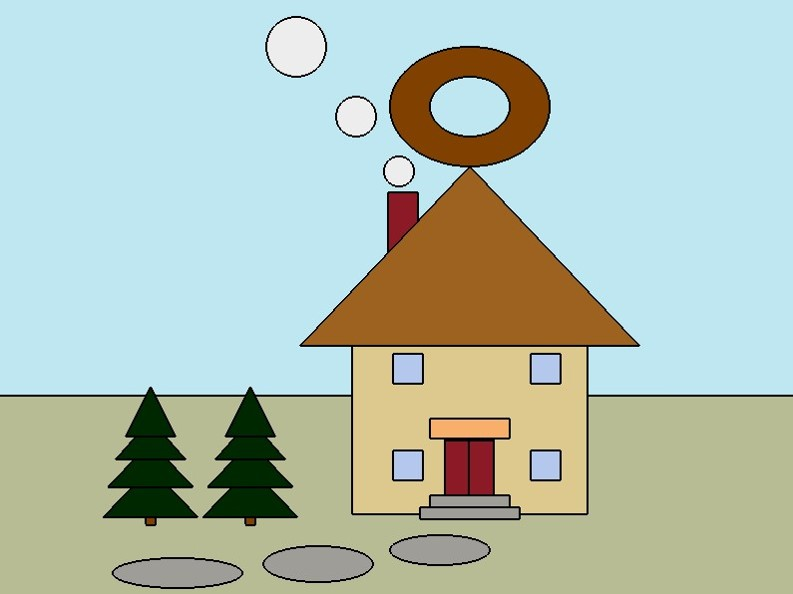
\includegraphics[width=0.8\textwidth]{figure/chap06/09shapehouse}};
    
    \end{tikzpicture}
  \end{center}  
\end{frame}

\begin{frame}[t, fragile]{抽象类}{实例:甜甜圈小屋}%
  \begin{itemize}
  \item 例子: 甜甜圈小屋类设计
  \end{itemize}
  \begin{center}
     \begin{tikzpicture}[font=\tiny, show background grid]
      \tikzset{ coord/.style={coordinate} }

      \begin{class}[fill=red!25, text width=4em]{形状类CShape}{0, 0}

      \end{class}

      \begin{class}[fill=green!25, text width=6em]{等腰三角形类CTriangle}{-3, -2}
        \inherit{形状类CShape}

      \end{class}
      
      \begin{class}[fill=green!25, text width=4em]{矩形类CRectangle}{0, -2}
        \inherit{形状类CShape}

      \end{class}
      
      \begin{class}[fill=green!25, text width=4em]{椭圆类CEllipse}{3, -2}
        \inherit{形状类CShape}

      \end{class}

      \begin{class}[fill=blue!25, text width=4em]{长方体类CCuboid}{0, -4}
        \inherit{矩形类CRectangle}

      \end{class}

      \begin{class}[fill=blue!25, text width=4em]{圆环类CDonut}{3, -4}
        \inherit{椭圆类CEllipse}

      \end{class}
           
    \end{tikzpicture}    
  \end{center}
\end{frame}

\begin{frame}[t, fragile]{抽象类}{实例:甜甜圈小屋}%
  \begin{itemize}
  \item 例子: 甜甜圈小屋代码设计
  \end{itemize}
  %\vspace{-2ex}
  \begin{center}
     \begin{tikzpicture}[font=\tiny, show background grid]
       \tikzset{ coord/.style={coordinate} }

       \umlnote[scale = 0.90,text width=0.6\textwidth](code1) at (0, 0)
      {
        \cppfilettnobg{codes/chap06/08-abstract-Shape.h}
      };

      \path let \p1=(code1) in
      coordinate (org) at (\x1, \y1)
      coordinate (ovBL0) at ($(org) + (-3.3, -2.95)$)
      coordinate (ovUR0) at ($(ovBL0) + (2.5, 0.5)$)
      coordinate (ovBR0) at ($(ovBL0) + (2.5, 0.0)$)
      coordinate (ovfunc0) at ($(ovUR0)!0.5!(ovBR0)$)
      ;

      \draw[blue,thick,fill=red!35, fill opacity=0.3](ovBL0) rectangle
      (ovUR0);     
           
    \end{tikzpicture}    
  \end{center}
\end{frame}

\begin{frame}[t, fragile]{抽象类}{实例:甜甜圈小屋}%
  \begin{itemize}
  \item 例子: 甜甜圈小屋代码设计
  \end{itemize}
  \begin{center}
     \begin{tikzpicture}[font=\tiny, show background grid]
       \tikzset{ coord/.style={coordinate} }

       \umlnote[scale = 0.90,text width=0.6\textwidth](code1) at (0, 0)
      {
        \cppfilettnobg{codes/chap06/08-abstract-ShapeArr.h}
      };

      \path let \p1=(code1) in
      coordinate (org) at (\x1, \y1)
      coordinate (ovBL0) at ($(org) + (-3.30, -0.25)$)
      coordinate (ovUR0) at ($(ovBL0) + (3.0, 0.3)$)
      coordinate (ovBR0) at ($(ovBL0) + (3.0, 0.0)$)
      coordinate (ovMR0) at ($(ovUR0)!0.5!(ovBR0)$)
      ;

      \node[fill=blue!25, draw, right=0.3 of ovMR0] (note1) {基类类型指针
        数组};

      \path let \p1=(code1) in
      coordinate (org) at (\x1, \y1)
      coordinate (ovBL1) at ($(org) + (-3.30, -1.20)$)
      coordinate (ovUR1) at ($(ovBL1) + (2.18, 0.3)$)
      coordinate (ovBR1) at ($(ovBL1) + (2.18, 0.0)$)
      coordinate (ovMR1) at ($(ovUR1)!0.5!(ovBR1)$)
      ;

      \node[fill=blue!25, draw, right=0.3 of ovMR1] (note1) {基类类型指针
        形参};

      \draw[blue,thick,fill=red!35, fill opacity=0.3](ovBL0) rectangle
      (ovUR0);
      \draw[blue,thick,fill=red!35, fill opacity=0.3](ovBL1) rectangle
      (ovUR1); 
           
    \end{tikzpicture}    
  \end{center}
\end{frame}

\begin{frame}[t, fragile]{抽象类}{实例:甜甜圈小屋}%
  \begin{itemize}
  \item 例子: 甜甜圈小屋代码设计
  \end{itemize}
  \begin{center}
     \begin{tikzpicture}[font=\tiny, show background grid]
       \tikzset{ coord/.style={coordinate} }

       \umlnote[scale = 0.90, text width=0.6\textwidth](code1) at (0, 0)
      {
        \cppfilettnobg{codes/chap06/08-abstract-ShapeArr.cpp}
      };

      \path let \p1=(code1) in
      coordinate (org) at (\x1, \y1)
      coordinate (ovBL0) at ($(org) + (-3.05, 0.85)$)
      coordinate (ovUR0) at ($(ovBL0) + (1.89, 0.30)$)
      coordinate (ovBR0) at ($(ovBL0) + (1.89, 0.00)$)
      coordinate (ovMR0) at ($(ovUR0)!0.5!(ovBR0)$)
      ;

      \node[fill=blue!25, draw, text width=0.3\textwidth, right=2 of ovMR0] (note1) {基类类型
        指针指向派生类对象,\alert{调用派生类中的函数}};

      \path let \p1=(code1) in
      coordinate (org) at (\x1, \y1)
      coordinate (ovBL1) at ($(org) + (-3.05, -0.80)$)
      coordinate (ovUR1) at ($(ovBL1) + (2.14, 0.30)$)
      coordinate (ovBR1) at ($(ovBL1) + (2.14, 0.00)$)
      coordinate (ovMR1) at ($(ovUR1)!0.5!(ovBR1)$)
      ;

      \path let \p1=(code1) in
      coordinate (org) at (\x1, \y1)
      coordinate (ovBL2) at ($(org) + (-3.05, -2.45)$)
      coordinate (ovUR2) at ($(ovBL2) + (2.62, 0.30)$)
      coordinate (ovBR2) at ($(ovBL2) + (2.62, 0.00)$)
      coordinate (ovMR2) at ($(ovUR2)!0.5!(ovBR2)$)
      ;

      \draw[blue,thick,fill=red!35, fill opacity=0.3](ovBL0) rectangle
      (ovUR0);
      \draw[blue,thick,fill=red!35, fill opacity=0.3](ovBL1) rectangle
      (ovUR1);
      \draw[blue,thick,fill=red!35, fill opacity=0.3](ovBL2) rectangle
      (ovUR2);

      \draw[-{Stealth[scale=1.0]}, red, thick] (ovMR0) to[out=0,
      in=180] (note1.west);
      \draw[-{Stealth[scale=1.0]}, red, thick] (ovMR1) to[out=0,
      in=180] (note1.west);
      \draw[-{Stealth[scale=1.0]}, red, thick] (ovMR2) to[out=0,
      in=180] (note1.west);
           
    \end{tikzpicture}    
  \end{center}
\end{frame}

\begin{frame}[t, fragile]{抽象类}{实例:甜甜圈小屋}%
  \begin{itemize}
  \item 例子: 甜甜圈小屋代码设计
  \end{itemize}
  \begin{center}
     \begin{tikzpicture}[font=\tiny, show background grid]
       \tikzset{ coord/.style={coordinate} }

       \umlnote[text width=0.6\textwidth](code1) at (0, 0)
      {
        \cppfilettnobg{codes/chap06/08-abstract-dtor.cpp}
      };

      \path let \p1=(code1) in
      coordinate (org) at (\x1, \y1)
      coordinate (ovBL0) at ($(org) + (-3.10, -1.28)$)
      coordinate (ovUR0) at ($(ovBL0) + (2.25, 0.55)$)
      coordinate (ovBR0) at ($(ovBL0) + (2.25, 0.00)$)
      coordinate (ovMR0) at ($(ovUR0)!0.5!(ovBR0)$)
      ;

      \node[fill=blue!25, draw, text width=0.3\textwidth, right=0.3 of ovMR0] (note1) {基类类型
        指针指向派生类对象,\alert{调用派生类中的函数}};

      \draw[blue,thick,fill=red!35, fill opacity=0.3](ovBL0) rectangle
      (ovUR0);
           
    \end{tikzpicture}    
  \end{center}
\end{frame}

\begin{frame}[t, fragile]{抽象类}{实例:甜甜圈小屋}%
  \begin{itemize}
  \item 例子: 甜甜圈小屋-测试数据
  \end{itemize}
  \begin{center}
     \begin{tikzpicture}[font=\tiny, show background grid]
       \umlnote[text width=0.6\textwidth, scale=0.85] (code1) at (0, 0)
       {         
           \cppfilenobg{codes/chap06/08-abstract-data.cpp}
      };
    \end{tikzpicture}    
  \end{center}
\end{frame}

\begin{frame}[t, fragile]{抽象类}{实例:实践}%
  \stretchon
  \begin{itemize}
  \item 练习:形状类的设计
    \begin{itemize}
    \item 设计要求
      \begin{itemize}
      \item 设计一个CShape抽象类,类中包含纯虚函数
      \item 从CShape类派生出三角形类CTriangle、矩形类CRectangle和椭圆
        类CEllipse
      \item 使用一个公共接口计算三角形对象、矩形对象和椭圆对象面积之和
      \item 重载运算符>用于判断两个形状面积的大小,返回true或false
      \end{itemize}
    \end{itemize}
  \end{itemize}
  \stretchoff
\end{frame}

\begin{frame}[t, fragile]{抽象类}{RTTI}%
  \stretchon
  \begin{itemize}
  \item 运行时刻类型识别(RunTime Type Identification):允许使用基类指
    针或引用操纵对象的程序获得这些指针或引用实际所指对象的类型。
  \item \cppinlinett{dynamic_cast}运算符
  \item \cppinlinett{typeid}运算符
  \end{itemize}
  \stretchoff
\end{frame}

\begin{frame}[t, fragile]{抽象类}{C++的4种类型转换符}%
  \stretchon
  \begin{itemize}
  \item \cppinlinett{static_cast}
  \item \cppinlinett{dynamic_cast}
    \begin{itemize}
    \item 向下类型转换
    \end{itemize}
  \item \cppinlinett{reinterpret_cast}
  \item \cppinlinett{const_cast}
  \end{itemize}
  \stretchoff
\end{frame}

\begin{frame}[t, fragile]{抽象类}{\cppinlinett{dynamic_cast}}%
  \begin{itemize}
  \item 向下类型转换
  \end{itemize}
  \begin{center}
     \begin{tikzpicture}[font=\tiny, show background grid]
       \tikzset{ coord/.style={coordinate} }

       \umlnote[text width=0.6\textwidth](code1) at (0, 0)
      {
        \cppfilettnobg{codes/chap06/09-rtti-class.cpp}
      };

      \umlnote[text width=0.55\textwidth, right=-2.3 of code1](code2)
      {
        \cppfilettnobg{codes/chap06/09-rtti-fun.cpp}
      };

      \path let \p1=(code2) in
      coordinate (org) at (\x1, \y1)
      coordinate (ovBL0) at ($(org) + (-3.35, -0.27)$)
      coordinate (ovUR0) at ($(ovBL0) + (4.95, 0.3)$)
      coordinate (ovBR0) at ($(ovBL0) + (4.95, 0.0)$)
      coordinate (ovMR0) at ($(ovUR0)!0.5!(ovBR0)$)
      ;

      % \node[fill=blue!25, draw, text width=0.3\textwidth, right=0.3 of ovMR0] (note1) {基类类型
      %   指针指向派生类对象,\alert{调用派生类中的函数}};

      \draw[blue,thick,fill=red!35, fill opacity=0.3](ovBL0) rectangle
      (ovUR0);
           
    \end{tikzpicture}    
  \end{center}
\end{frame}

\begin{frame}[t, fragile]{抽象类}{\cppinlinett{typeid}}%
  \begin{itemize}
  \item 向下类型转换
  \end{itemize}
  \begin{center}
     \begin{tikzpicture}[font=\tiny, show background grid]
       \tikzset{ coord/.style={coordinate} }

       \umlnote[text width=0.6\textwidth](code1) at (0, 0)
      {
        \cppfilettnobg{codes/chap06/09-rtti-main.cpp}
      };

      \node[text width=0.3\textwidth, right=0.3 of code1] (fig1)
      {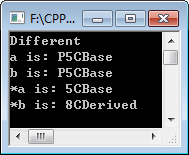
\includegraphics[width=0.8\textwidth]{figure/chap06/10rtti}};


      \path let \p1=(code1) in
      coordinate (org) at (\x1, \y1)
      coordinate (ovBL0) at ($(org) + (-4.0, 1.45)$)
      coordinate (ovUR0) at ($(ovBL0) + (2.15, 0.3)$)
      coordinate (ovBR0) at ($(ovBL0) + (2.15, 0.0)$)
      coordinate (ovMR0) at ($(ovUR0)!0.5!(ovBR0)$)
      ;

      \node[fill=blue!25, draw, text width=0.3\textwidth, above=0.3 of fig1] (note1) {编译器不同,输出可能不同!};

      \draw[blue,thick,fill=red!35, fill opacity=0.3](ovBL0) rectangle
      (ovUR0);
           
    \end{tikzpicture}    
  \end{center}
\end{frame}

\section[联编]{静态联编与动态联编}\label{sec:chap06-sec03}
%%%%%%%%%%%%%%%%%%%%%%%%%%%%%% 继承的方式 %%%%%%%%%%%%%%%%%%%%%%%%%%%%%%%%%%
\begin{frame}[t, fragile]{编译链接}{静态联编与动态联编}%
  \stretchon
  \begin{itemize}
  \item 静态联编(static binding or early binding)
    \begin{itemize}
    \item 在编译时确定同名函数的具体操作对象
      \begin{itemize}
      \item 重载函数
      \item 函数模板
      \item 运算符重载
      \end{itemize}
    \item 特点:执行效率高,但灵活性差
    \end{itemize}
  \item 动态联编(dynamic binding or late binding)
    \begin{itemize}
    \item 在程序运行时(run time)确定对象所调用的函数
      \begin{itemize}
      \item 虚函数
      \item 纯虚函数
      \end{itemize}
    \item 特点:灵活性强,但效率可能会降低
    \end{itemize}
  \end{itemize}
  \stretchoff
\end{frame}

\section[小结]{本章小结}\label{sec:chap06-sec04}
%%%%%%%%%%%%%%%%%%%%%%%%%%%%%% 继承的方式 %%%%%%%%%%%%%%%%%%%%%%%%%%%%%%%%%%
\begin{frame}[t]{小结}{本章小结}%
  \stretchon
  \begin{itemize}
  \item \alert{多态性}是面向对象程序设计的重要特性之一,多态是指同样的消息被不
    同类型的对象接收时导致完全不同的行为。
  \item \alert{虚函数}是在基类中定义的以virtual关键字作为开头的成员函数,需要
    在派生类中重新定义。
  \item \alert{纯虚函数}是一个在基类中声明的没有定义具体实现的虚函数,带有纯虚
    函数的类称为抽象类。
  \item \alert{抽象类}为一个类族提供统一的操作界面。抽象类处于类层次的上层,自
    身无法实例化,只能通过继承机制,生成抽象类的具体派生类,然后再实例
    化。通过抽象类的指针和引用,可以指向并访问各派生类成员,实现多态性。
  \item 联编可以在编译和连接时进行,称为\alert{静态联编};联编也可以在运行时进行,称为\alert{动态联编}。
  \end{itemize}
  \stretchoff
\end{frame}

%%%%%%%%%%%%%%%%%%%%%%%%%%%%%%%%%%%%%%%%%%%%%%%%%%%%%%%%%%%%%%%%%%%%%%%%%%%%%%%
% 附件页
\section[附件下载]{本讲示例代码及附件下载} 
\begin{frame}{附件}{本讲附件}
  % 此处的[ucfilespec=...]必须指定为pdf否则Windows下无法下载
  %\vspace{-4ex}
  \textattachfile[ucfilespec=ex-src06.pdf]{ex-src06.zip}{附件:右键单击该
    链接,选择\qtmark{\alert{保存附件}}下载,\alert{将后缀名改为\qtmark{.zip}解压}
      \footnote[frame]{请\alert{退出全屏模式}后点击该链接。}
      \footnote[frame]{以Adobe Acrobat Reader为例。}
      。}%\\

  \vspace{-1ex}
  \begin{center}
    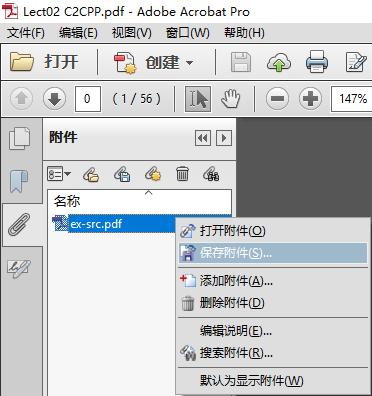
\includegraphics[height=0.35\textheight]{pdfattatchdownload01}\quad
    %或 \quad%
    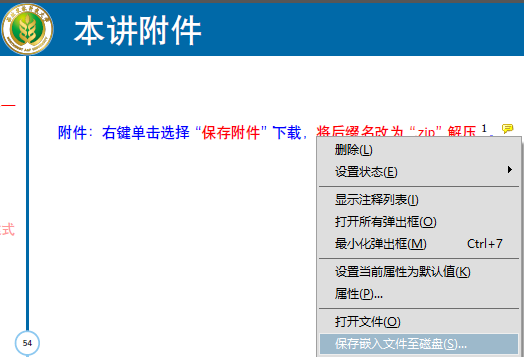
\includegraphics[height=0.35\textheight]{pdfattatchdownload02}\\[2ex]%
    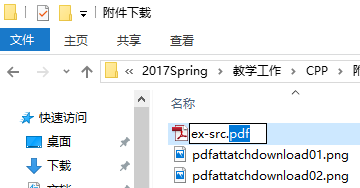
\includegraphics[height=0.255\textheight]{pdfattatchdownload03}\quad
    %$\Rightarrow$ \quad%
    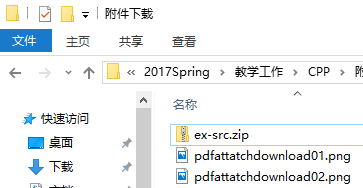
\includegraphics[height=0.255\textheight]{pdfattatchdownload04}%
  \end{center}   
\end{frame}

% \tiny
% \scriptsize
% \footnotesize
% \small
% \normalsize
% \large
% \Large
% \LARGE
% \huge
% \Huge


%%% Local Variables: 
%%% mode: latex
%%% TeX-master: "../main.tex"
%%% End: 
